% This file was created with tikzplotlib v0.10.1.
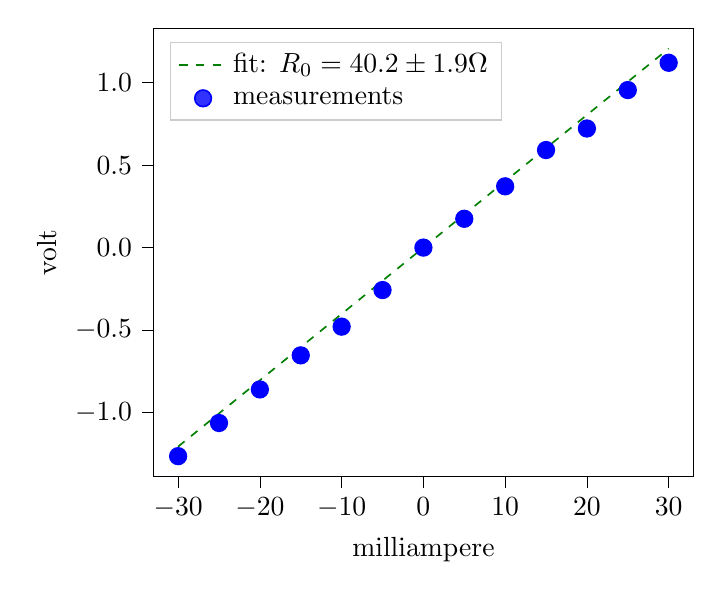
\begin{tikzpicture}

\definecolor{darkgray176}{RGB}{176,176,176}
\definecolor{green01270}{RGB}{0,127,0}
\definecolor{lightgray204}{RGB}{204,204,204}

\begin{axis}[
legend cell align={left},
legend style={
  fill opacity=0.8,
  draw opacity=1,
  text opacity=1,
  at={(0.03,0.97)},
  anchor=north west,
  draw=lightgray204
},
tick align=outside,
tick pos=left,
x grid style={darkgray176},
xlabel={milliampere},
xmin=-33, xmax=33,
xtick style={color=black},
xtick={-40,-30,-20,-10,0,10,20,30,40},
xticklabels={
  \(\displaystyle {\ensuremath{-}40}\),
  \(\displaystyle {\ensuremath{-}30}\),
  \(\displaystyle {\ensuremath{-}20}\),
  \(\displaystyle {\ensuremath{-}10}\),
  \(\displaystyle {0}\),
  \(\displaystyle {10}\),
  \(\displaystyle {20}\),
  \(\displaystyle {30}\),
  \(\displaystyle {40}\)
},
y grid style={darkgray176},
ylabel={volt},
ymin=-1.38750510988697, ymax=1.32960730762637,
ytick style={color=black},
ytick={-1.5,-1,-0.5,0,0.5,1,1.5},
yticklabels={
  \(\displaystyle {\ensuremath{-}1.5}\),
  \(\displaystyle {\ensuremath{-}1.0}\),
  \(\displaystyle {\ensuremath{-}0.5}\),
  \(\displaystyle {0.0}\),
  \(\displaystyle {0.5}\),
  \(\displaystyle {1.0}\),
  \(\displaystyle {1.5}\)
}
]
\path [draw=blue, semithick]
(axis cs:-30.1,-1.264)
--(axis cs:-29.9,-1.264);

\path [draw=blue, semithick]
(axis cs:-25.1,-1.063)
--(axis cs:-24.9,-1.063);

\path [draw=blue, semithick]
(axis cs:-20.1,-0.8595)
--(axis cs:-19.9,-0.8595);

\path [draw=blue, semithick]
(axis cs:-15.1,-0.653)
--(axis cs:-14.9,-0.653);

\path [draw=blue, semithick]
(axis cs:-10.1,-0.479)
--(axis cs:-9.9,-0.479);

\path [draw=blue, semithick]
(axis cs:-5.1,-0.2572)
--(axis cs:-4.9,-0.2572);

\path [draw=blue, semithick]
(axis cs:-0.1,0)
--(axis cs:0.1,0);

\path [draw=blue, semithick]
(axis cs:4.9,0.1748)
--(axis cs:5.1,0.1748);

\path [draw=blue, semithick]
(axis cs:9.9,0.3714)
--(axis cs:10.1,0.3714);

\path [draw=blue, semithick]
(axis cs:14.9,0.5913)
--(axis cs:15.1,0.5913);

\path [draw=blue, semithick]
(axis cs:19.9,0.7218)
--(axis cs:20.1,0.7218);

\path [draw=blue, semithick]
(axis cs:24.9,0.9548)
--(axis cs:25.1,0.9548);

\path [draw=blue, semithick]
(axis cs:29.9,1.1202)
--(axis cs:30.1,1.1202);

\path [draw=blue, semithick]
(axis cs:-30,-1.314)
--(axis cs:-30,-1.214);

\path [draw=blue, semithick]
(axis cs:-25,-1.113)
--(axis cs:-25,-1.013);

\path [draw=blue, semithick]
(axis cs:-20,-0.9095)
--(axis cs:-20,-0.8095);

\path [draw=blue, semithick]
(axis cs:-15,-0.703)
--(axis cs:-15,-0.603);

\path [draw=blue, semithick]
(axis cs:-10,-0.529)
--(axis cs:-10,-0.429);

\path [draw=blue, semithick]
(axis cs:-5,-0.3072)
--(axis cs:-5,-0.2072);

\path [draw=blue, semithick]
(axis cs:0,-0.05)
--(axis cs:0,0.05);

\path [draw=blue, semithick]
(axis cs:5,0.1248)
--(axis cs:5,0.2248);

\path [draw=blue, semithick]
(axis cs:10,0.3214)
--(axis cs:10,0.4214);

\path [draw=blue, semithick]
(axis cs:15,0.5413)
--(axis cs:15,0.6413);

\path [draw=blue, semithick]
(axis cs:20,0.6718)
--(axis cs:20,0.7718);

\path [draw=blue, semithick]
(axis cs:25,0.9048)
--(axis cs:25,1.0048);

\path [draw=blue, semithick]
(axis cs:30,1.0702)
--(axis cs:30,1.1702);

\addplot [semithick, green01270, dashed]
table {%
-30 -1.2061021977394
-25 -1.00508516478283
-20 -0.804068131826268
-15 -0.603051098869701
-10 -0.402034065913134
-5 -0.201017032956567
0 0
5 0.201017032956567
10 0.402034065913134
15 0.603051098869701
20 0.804068131826268
25 1.00508516478283
30 1.2061021977394
};
\addlegendentry{fit: $R_0 = 40.2 \pm 1.9\Omega$}
\addplot [semithick, blue, mark=*, mark size=3, mark options={solid}, only marks]
table {%
-30 -1.264
-25 -1.063
-20 -0.8595
-15 -0.653
-10 -0.479
-5 -0.2572
0 0
5 0.1748
10 0.3714
15 0.5913
20 0.7218
25 0.9548
30 1.1202
};
\addlegendentry{measurements}
\end{axis}

\end{tikzpicture}
